{\color{gray}\hrule}
\begin{center}
\section{Visual Analysis}
\textbf{Visual Analysis}
\bigskip
\end{center}
{\color{gray}\hrule}
\begin{multicols}{2}
\subsection{Area Conservation}
To analyze the behaviour of the soft body, one of the things I looked at was the evolution of area of the soft body as it interacts with it's surroundings via collision.
\begin{center}
    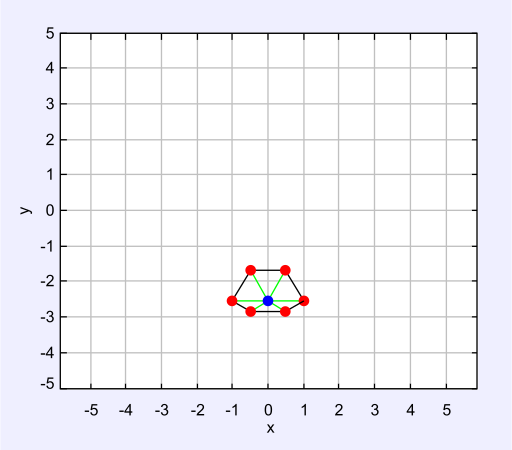
\includegraphics[scale=0.5]{media/visualAnalysis/areaConsv/deformation11.pdf}\\

    \includegraphics[scale=0.5]{media/visualAnalysis/areaConsv/deformation12.pdf}\\
    \includegraphics[scale=0.5]{media/visualAnalysis/areaConsv/deformation13.pdf}\\
    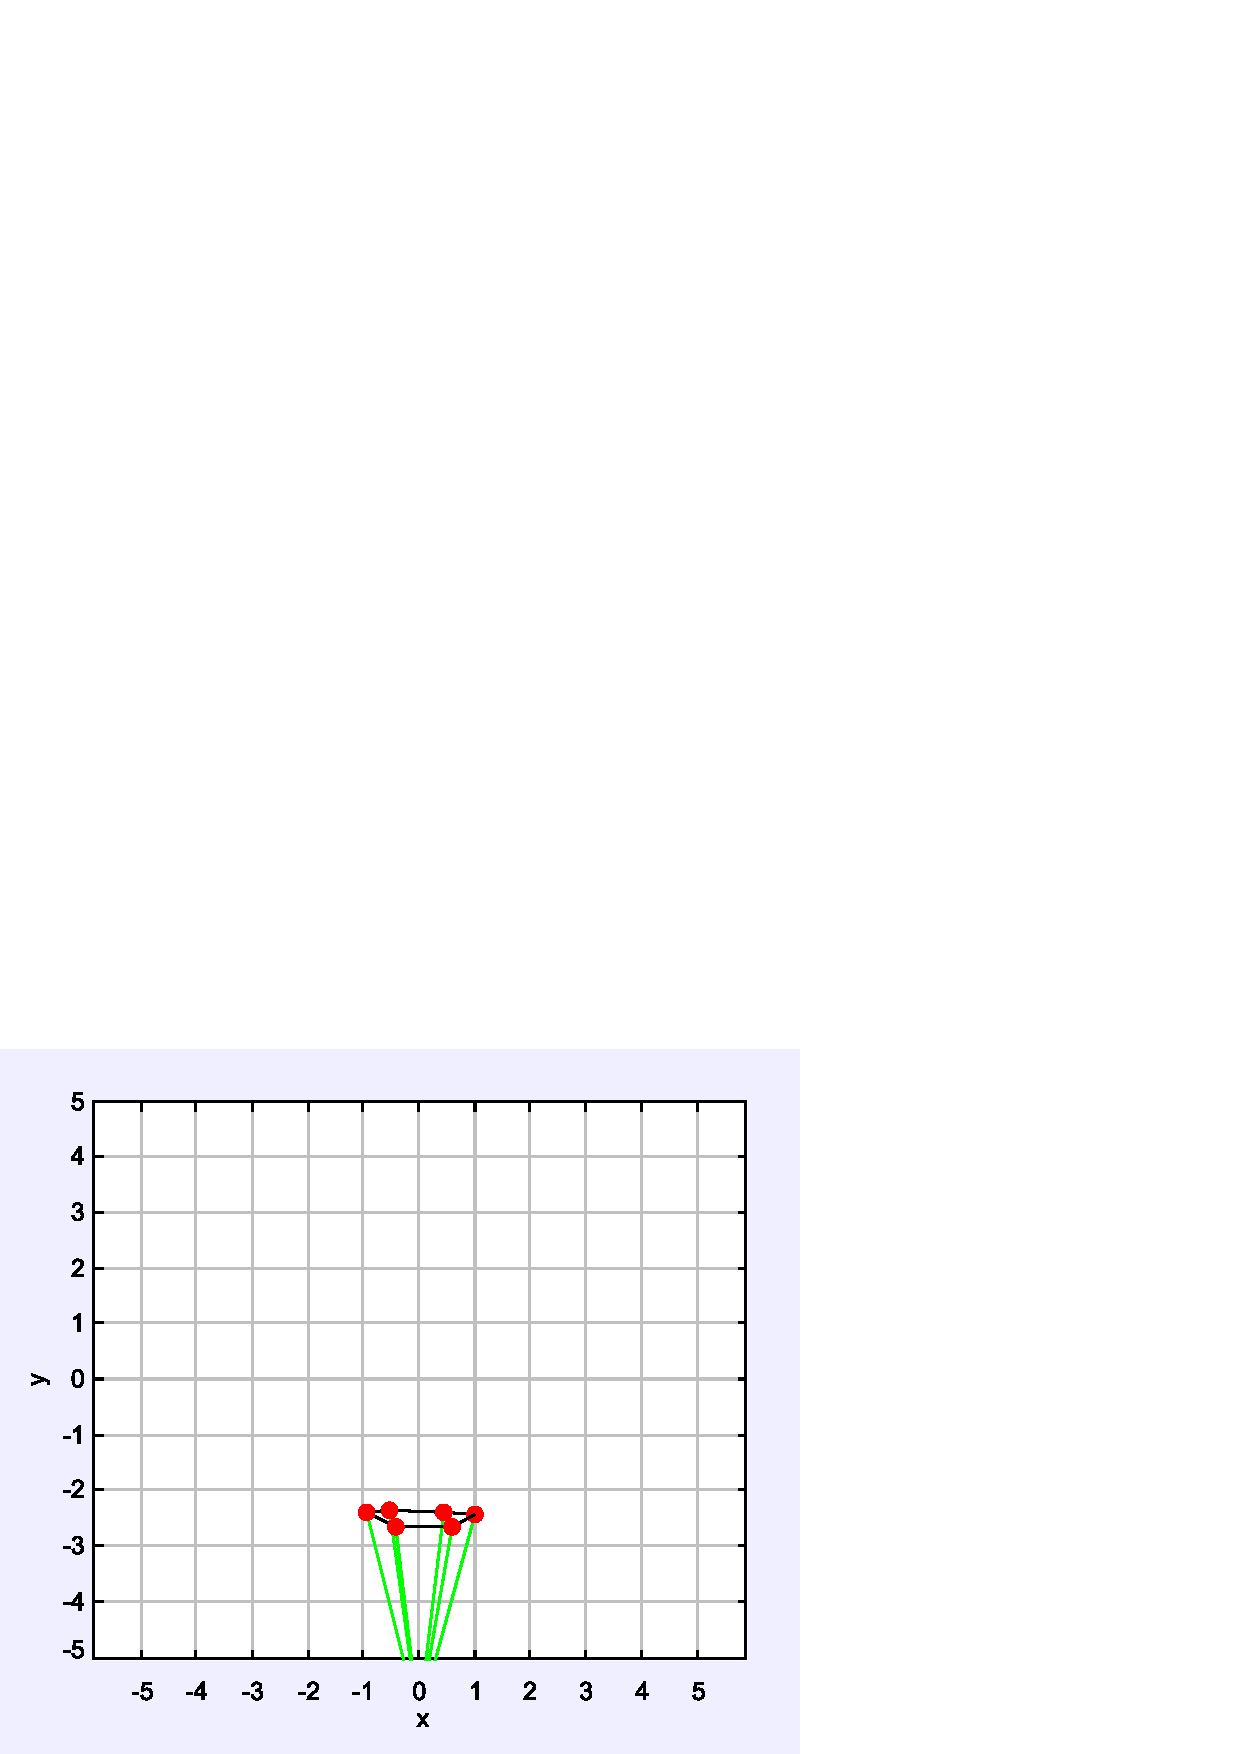
\includegraphics[scale=0.5]{media/visualAnalysis/areaConsv/deformation14.pdf}\\
\end{center}

As can be seen in the images, the shape of the soft body is not conserved and deforms significantly on collision.
\begin{center}
    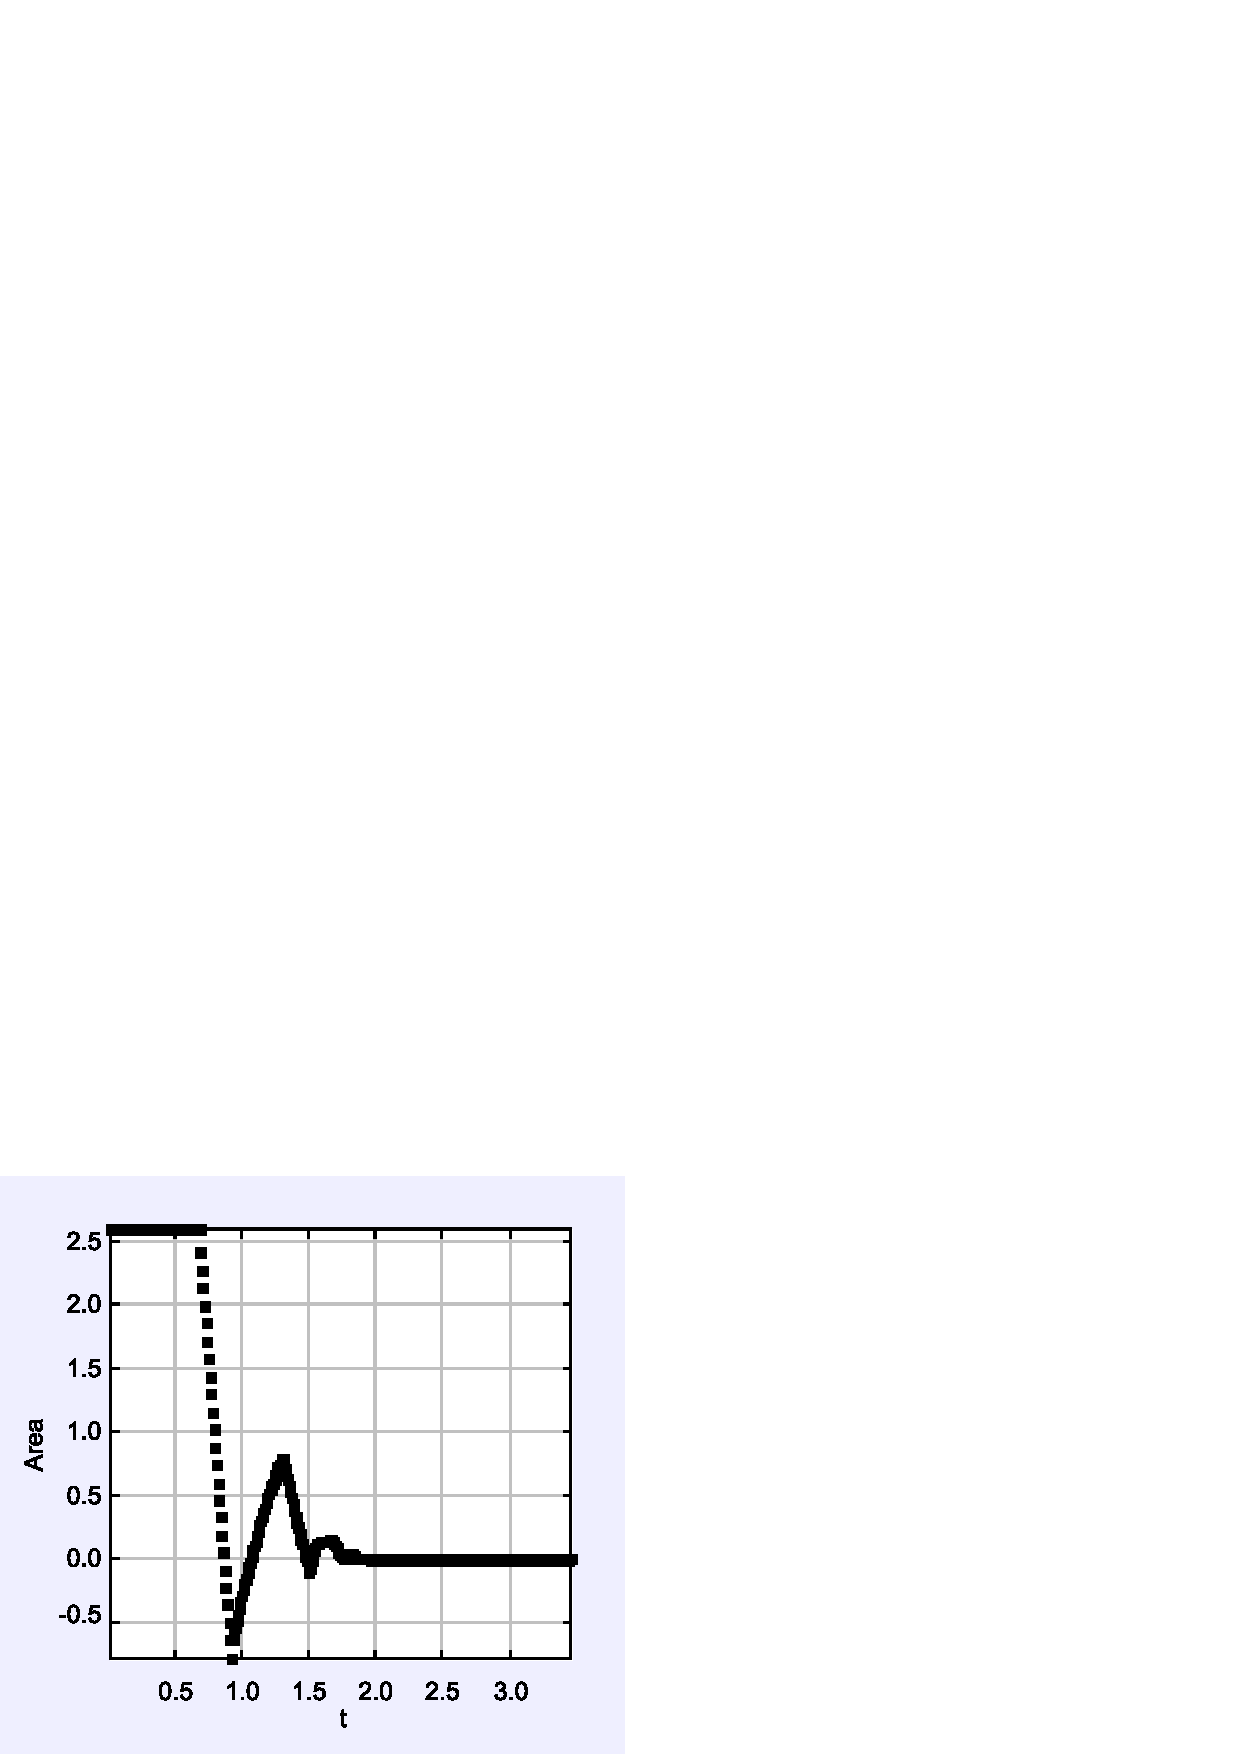
\includegraphics[scale=0.5]{media/visualAnalysis/areaConsv/deformation1areaTime.pdf}
\end{center}
\subsection{Subsection}
\lipsum[1-3]
\end{multicols}